\section{Related Works}

% http://se-pubs.dbs.uni-leipzig.de/

During our investigation, we found different approaches to the problematic, some of them bring some solution with tools and the other ones are only best practices and processes. None of them have solved our requirements entirely even if we found a lot of ideas that we have used intuitively before reading the papers or that we have integrate since we discovered them. We will start to describe the process oriented papers and after that the tools.

\subsection{Database refactoring}

In software engineering, the concept of code refactoring is well known and has become a standard practice. According to Fowler \cite{fowler_evolutionary}, refactoring is defined as \emph{``the process of changing a software system in such a way that it does not alter the external behavior of the code yet improves its internal structure''}. Code refactoring is an important practice in agile software development. It encourages programmers to start with a system design that is as simple as possible, and to add complexity iteratively in response to new requirements. Code refactoring is closely related to unit testing, because having a collection of automated tests makes the refactoring process much less risky (running the tests is a way to verify that the external behavior has not been affected by the refactoring).

In \cite{ambler_process_2011}, Ambler has introduced the related notion of \emph{``database refactoring''}, with the following definition: \begin{quote}\textit{A database refactoring is a small change to your database schema which improves its design without changing its semantics (e.g. you don't add anything nor do you break anything).  The process of database refactoring is the evolutionary improvement of your database schema so as to improve your ability to support the new needs of your customers, support evolutionary software development, and to fix existing legacy database design problems.}\end{quote}

Ambler explains that a database refactoring can be more or less difficult, depending on the number of applications built on top of the database. When a single application is built on top of the database, the impact can be relatively easy to assess. When several applications are built on top of the database, the impact analysis is much more complex. This is particularly true if the applications are managed by different organizations. Of course, whether or not the applications built on top of the database are covered by unit tests makes a huge difference when it comes to measure the impact of a refactoring.

Ambler describes database refactoring as a three-step process. The process starts in the development sandbox, is implemented in the integration sandbox and finally installed into production. While initiating the work in the development sandbox, the developer should go through a sequence of well-defined steps. After assessing the need to perform the refactoring, developers should implement unit tests, write schema modification and data transformation scripts, run tests and make sure that their scripts are under version control. Ambler also refers to an interesting idea, introduced by Sadalage and Schuh \cite{sadalage_agile_database}: the notion of a \emph{deprecation} (or \emph{transition}) \emph{period}. The idea is that a change in the database schema cannot be taken into account immediately by all applications. During the transition period, all applications should still work, some of them using the new schema and others using the old one. Mechanisms, such as triggers, can be used to keep the data consistent under such circumstances.

Our framework has several elements in common with the process described by Ambler. Firstly, it also describes concrete procedures, with well-defined steps, that have to be followed by developers (i.e. it is quite prescriptive). Secondly, it has been developed in an agile development organization. New requirements are frequent, and so are the are the needs to perform database transformations.

\subsection{Migration process}

David Katzoff \cite{katzoff_how_2011} offers a solution to test the data migrations. First of all, he demonstrates that the sampling approach is not suitable for all the cases. With this approach, not all the data are verified that will not ensure all the data keep their integrity. He proposes to do Pre-Migration testing that brings a couple of actions before any migration procedure, followed by a Formal Design Review that describe the source and target systems, quantity of migrations (data, queries, ...), resources required, time required and so on. After that, Post-Migration Testing are done to detect any defect. These tests are done on a sandbox environment that is specific for data migration and allow testing. Finally, the User Acceptance Testing could be done to detect any other defects that could not be found automatically. Once these tests are done, the Production Migration is ready to be done. Finally, David Katzoff offers ten recommendations to handle data migrations from process point of view.

This methodology is specially appreciated when your software development process is planned on a relative long period (more than two weeks). In our case, we use the SCRUM\cite{schwaber_agile_2002}, \cite{scrum} methodology to manage our development. In this methodology, we organize our develiveries in terms of sprints of two weeks duration. In other terms, it means that we could potentially have migrations every two weeks. We cannot manage such a process as propose by David Katzoff due to the people implied in the process and the time potentially consumed. We need to keep as most as possible the agility to add new features with data migration and keep confidence in the application and migrations. In this situation, we need to find a lightweight process to reach a balance between high modifications of data and stability of the applications. 

\subsection{MeDEA}

Metamodel-based Database Evolution Architecture (MeDEA)\cite{Dominguez2008419} offers a generic evolution architecture to maintain the traceability between the different elements involved in database development process. This method is generic because it does not use a specific modeling technique as an input. In the whole system, a translation component between conceptual schemas and logical schemas is used. This is the principal contribution of this approach. The translation element does the conversion between the conceptual and logical schemas with avoiding to start from scratch each conversion. The article concludes with the fact that the system is not designed for huge database with too many data. In this case, the performance and duration during a migration could be really awful.

This methodology brings is specially interesting for the fact that the modifications are planned with a metamodel. They are kept to trace each change in the database. It is designed in a way that any modeling language could be use to prepare the evolution. In our situation, such a system, is not totally appreciated. Some our refactoring implies some unplanned data model modification with an impact on the database schema. This situation required some reverse engineering approach to prepare the migration statements. MeDEA does not offer such a way to track these kind of modifications. One thing that we believe in is the traceability of the data migrations. For that, we want a system with the capability to track the modification to apply and the modification applied. For that, we need a structured approach that could be inspired by systems like MeDEA.

\subsection{DB-MAIN}

DB-MAIN\cite{Hick2006534} approach as the same kind of approach as MeDEA. The approach is centered on the evolution process and tries to address the problems of automatization of the database modifications. The article presents where the modification come from. The modifications come from a specification point of view. The whole solution analyze the way to track and apply the modification on the database and also on the application. One question asked is how to update an application after the database is updated to match the new specifications. One another interesting aspect this paper is the way to manage the modification tracking done by the migration. The history mechanism allows undoing the migrations. Idea is to write the reverse statement (includes all details required for that) that allows coming from a migrated version to an earlier version. There are also some recommendations like when a primary reference is introduced against existent data, the data present must be checked to be safe for the migration. It means that the foreign keys must satisfy the unique constraint check. The authors do the statement that the migrations for renaming, adding relations, attributes, entities or updating a cardinality are more frequent than conceptual refactoring. It means that the impact of such a modification has a less impact than the others. The paper gives the impact of database modification on the programs. For example, adding an attribute is quite transparent for an application.

One more time, the approach of this article comes from the conceptualization of the data store to the application. We do not want to go through this kind of process. Our applications run the process of database modeling through a data binding done by the frameworks we use. In this situation, we cannot apply directly the recommendations, processes and tools describe in this paper but we can study some aspects and use some of them. For example, the way that the history is used with the possibility to rollback any modifications done in a migration is really grateful. The traceability is the key concept to keep an ease of the data migration process. We try to address this at the beginning when the application is modified to the migration executed when the application is deployed. We have also defined the categorizes and risk levels for data migration types. As we have seen for now is that we have a lot of small migrations as the article describes and small amount of major migrations that could have a major impact during the migration execution.

\subsection{PRISM}

The PRISM \cite{curino_prism_2011} tool provides a language to define the migration changes. This language is called SMO\cite{smo} is a language that is not so far from SQL language. You can write the same kind of commands with additional ones. For example, you can write a command to split a table into two tables with \textit{DECOMPOSE TABLE objectcache INTO ob1(keyname, value), ob2(keyname, exptime);}. The figure~\ref{smoLanguage} shows the different commands and translation to relational language. The process used by the tool is defining the SMO queries to update the database schema, viewing the reverse queries (built on the base of forward queries), validating the queries (migration validation) and finally, running the migration (observing the queries).

\begin{figure}[h]
        \centering
        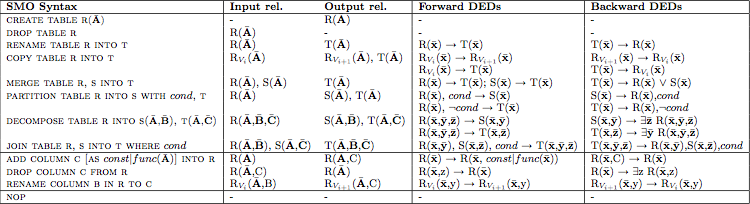
\includegraphics[scale=0.53]{images/Smo-to-ded.png}
        \caption{SMO Language for PRISM \cite{curino_prism_2011}}
        \label{smoLanguage}
\end{figure}

With PRISM, the changes to do must be well known before using the tool. In our case, we use an ORM that masquerade the changes and force us to find a way to detect the changes and which are they. In such a situation, it begins to be more difficult to use a tool to write the changes and one another to detect the changes. In this situation, we cannot use directly such a tool to manage our data migration.

\subsection{DBDeploy}

DBDeploy\cite{ashley_taking_2011} is a tool that provide a way to manage database migrations. The tools offer a way to check a database, retrieve the actual state and build the migration script ready to be run on test environment or production environment. The tool retrieve the actual state of a database directly from the database through a dedicated table that triggers the database evolutions. From there, it has the possibility to create the migration script from the current state to the state wanted by the developer modifications. The author, Nick Ashley, of the tool, describes best practices based partially on the "Database Refactoring" from Scott W. Ambler and also on what Martin Fowler advocates. In summary, it is recommended to work is small unit of change, committing frequently will avoid "check-in Friday" syndrome. Ashley says: "The use of a Continuous IntegrationI\cite{fowler_continuous_integration} tool is core to this method of database refactoring. Building functionality by small steps and rigorously building, deploying and testing the output at every step helps to raise bugs and other integration issues early and as so provide more time for them to be fixed in a more controllable manner." The white paper is based on ant for the usage of the tool but it exists also a Maven\cite{maven} plugin that the documentation could be found on the source code repository\cite{dbdeploy_source}.

One interesting fact in the approach of DBDeploy is the way to store the state of migration script ran into a certain database. The tool has its own table to monitor the database changelog. With this table, it becomes possible to follow the lifecycle of the database. It is possible to store the last migration script ran and the previous ones. Actually, we do not have such a method but it is something that we want to improve. We need a mechanism to monitor which scripts are run and where. Another interesting point, that we actually apply, is the way to manage the migration scripts. For DBDeploy approach, each change to the database \emph{must} have its own atomic script. It means that for each change done in the code must be reflected by a migration even if the change occurs in a short period. As Ashley said, the main point is organized around the CI tools. For us, we also have the same spirit about this kind of tools. We move towards a solution of a nightly build and testing for the specific field of database evolution in addition of our other testing processes.

As DBDeploy looks sexy, it does not address all the needs we are looking for. Actually, we do not need a tool to handle the construction of a final migration script, we already have one home made tool to do that. We need to add a way to know the current state of a specific database and to which state we want to go. Another tool we need is a tool to compare two database and see the delta between them in the context of continuous integration. 

\subsection{MoDEF}

MoDEF\cite{Terwilliger:2010:WDU:1807167.1807316} is an additional built in tool for the IDE\cite{ide} VisualStudio. It brings the capability to automatically writing the migration scripts to evolve a data store when a code change is detected (saved) on the disk in the context of data mapping framework. The tools offers automatism to prepare statements to migrate a database and in this situation, offers a bridge between database administrators and developers. They could discuss on a common base. The tool store the scripts when the code is saved on the hard disk under a log format. The developer can at any time generating the whole script, creation until latest modification, or upgrade a point in the code to the latest modification. The generated script contains comments relative to the updates done in the code that allows following the modifications.

This tool is really promising but only available for Visual Studio and for a specific data mapping framework. It is difficult to adapt it directly to other technologies but this is not the most blocking point. The tool and approach focuses the mapping changes or entity changes in general but the modifications of the data inside the data store is not handled and you could miss some changes that requires a data modification when the application is deployed. One example of this kind of non-monitoring changes could be when you store XML\cite{xml} in your database (the reason will not be discussed there) and you want to change the format of your XML stored in the database. Your schema remains exactly the same after your refactoring of the XML format but your application would not work anymore if you do not apply some data transformation to reflect your XML format change. MoDEF have no way to handle this kind of changes.

One interesting thing in this paper is the way that the modifications are viewed in terms of migration scripts. The atomicity principle for the modification scripts are applied. It means that for each code modification, a log entry is written (only if the code is saved) and a scripts could be generated for the modification. If the modification is reverted later with a new update of the code, another log entry is written for this modification. So another script could be generated to cancelled the previous one. In terms of semantic, each action on the code is logged and a scripts could be applied. In terms of application behavior and migration scripts, some changes could have no effect due to a counter-part script that cancel the previous one.



